\chapter{Ice Reservoirs}

\section{Introduction}

\begin{figure}[t]
\centering
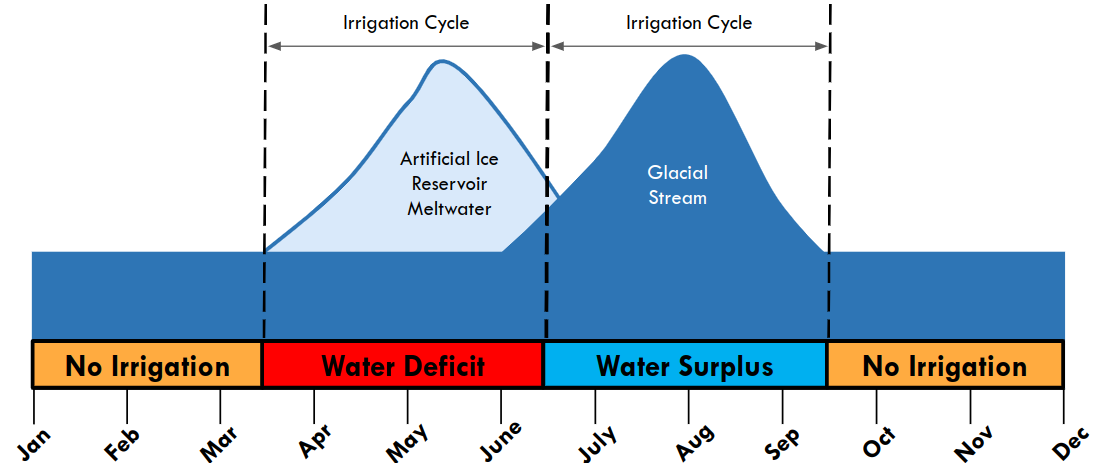
\includegraphics[width=12cm]{Figures/irrigation_cycles.png}

\caption{Seasonal variation in the availability of irrigation water. The graph highlights the crucial role of
AIRs in bridging the critical gap in water availability. Adapted from: \cite{nusserLocalKnowledgeGlobal2016}}

\label{fig:irrigation_cycles}
\end{figure}

Cryosphere-fed irrigation networks in arid mountain regions are completely dependent on the timely availability of
meltwater from glaciers, snow and permafrost \citep{immerzeelImportanceVulnerabilityWorld2020,
farhanHydrologicalRegimesConjunction2015, tveitenGlacierGrowingLocal2007}. With the accelerated decline of
glaciers due to climate change \citep{nusserLocalKnowledgeGlobal2016}, these regions are experiencing water
scarcity, particularly during spring \citep{norphelSnowWaterHarvesting2015,
mukhopadhyayReevaluationSnowmeltGlacial2015} (see Fig. \ref{fig:irrigation_cycles}). This seasonal water
scarcity warrants supplementary irrigation in order to sustain agricultural output and utilize the complete growing season \citep{nusserLocalKnowledgeGlobal2016, vincentEnergyClimateChange2009}.

To cope with this recurrent water scarcity, villagers in Ladakh have developed two types of
artificial ice reservoirs (AIRs): ice stupas and ice terraces. Both the ice reservoirs capture water
in the autumn and winter, allowing it to freeze, and hold it until spring, when it melts and flows down to
the fields \citep{ipccChapterHighMountain2019, vinceGlacierMan2009, clouseLadakhArtificialGlaciers2017,
nusserSociohydrologyArtificialGlaciers2019}. In this way, they retain a previously unused portion of the annual
flow and facilitate its use to supplement the decreased flow in the next spring (see Fig.
\ref{fig:irrigation_cycles}). This study focuses on one form of AIRs that are locally called "ice stupas".

Over the past decade, several ice stupas have been built to supplement irrigation water supply of mountain
villages in India \citep{wangchukIceStupaCompetition2020, palmerStoringFrozenWater2022,
aggarwalAdaptationClimateChange2021}, Kyrgyzstan \citep{bbcnewsBrightArtificialGlacier2020} and Chile
\citep{reutersConservationistsChileAim2021}. Despite this widespread adoption, only a few publications examine
the role of AIRs in the water resource management of these regions. None of these publications study AIRs
outside Ladakh. Moreover, the published quantifications of the water storage capacity of AIRs just in Ladakh
also vary widely between these studies \citep{norphelSnowWaterHarvesting2015, baglaArtificialGlaciersHelp1998}.

Quantifying the water storage capacity of AIRs is not straightforward since the formative processes of AIRs are
complex. These processes are controlled by local topography, meteorology and construction strategies used.
However, methodologies used to quantify meteorological influences on glaciers may also be applicable on these
ice reservoirs since their surface processes are similar. But due to their limited size, and comparatively more
variable surface area, this assessment requires a modelling approach which is optimally constrained with
comprehensive data from in-situ field measurements. 

A spirit of improvisation guides the construction strategies of AIRs. This has resulted in ice reservoirs
exhibiting significant volume variations despite experiencing similar meteorological conditions. For example,
ice terraces have attained volumes upto 30 times larger than ice stupas built in Ladakh, India
\cite{nusserSociohydrologyArtificialGlaciers2019}. However, the processes driving these differences can only be
resolved if the complete methodology of the construction strategy used is available.

This thesis fulfills both of these requirements as it provides a new set of AIR-specific volume and area
measurements from drone flights along with meteorological data during the construction period. All these
datasets were produced through construction strategies using fountain systems that are quantified via in-situ
observations of the fountain characteristics and discharge rate measurements. In a first step, this thesis
attempts to formulate a one-dimensional AIR model in order to calibrate and validate it with the AIR datasets.
In a second step, it attempts to use this model as a tool to propose a construction strategy designed to produce
AIRs efficiently and effortlessly. While this thesis reviews published AIR research and presents a comprehensive
quantitative study of their water storage potential, we acknowledge that substantial additional knowledge is
held by farming communities building these structures since mid-1800s.

\begin{figure}[t]
\centering
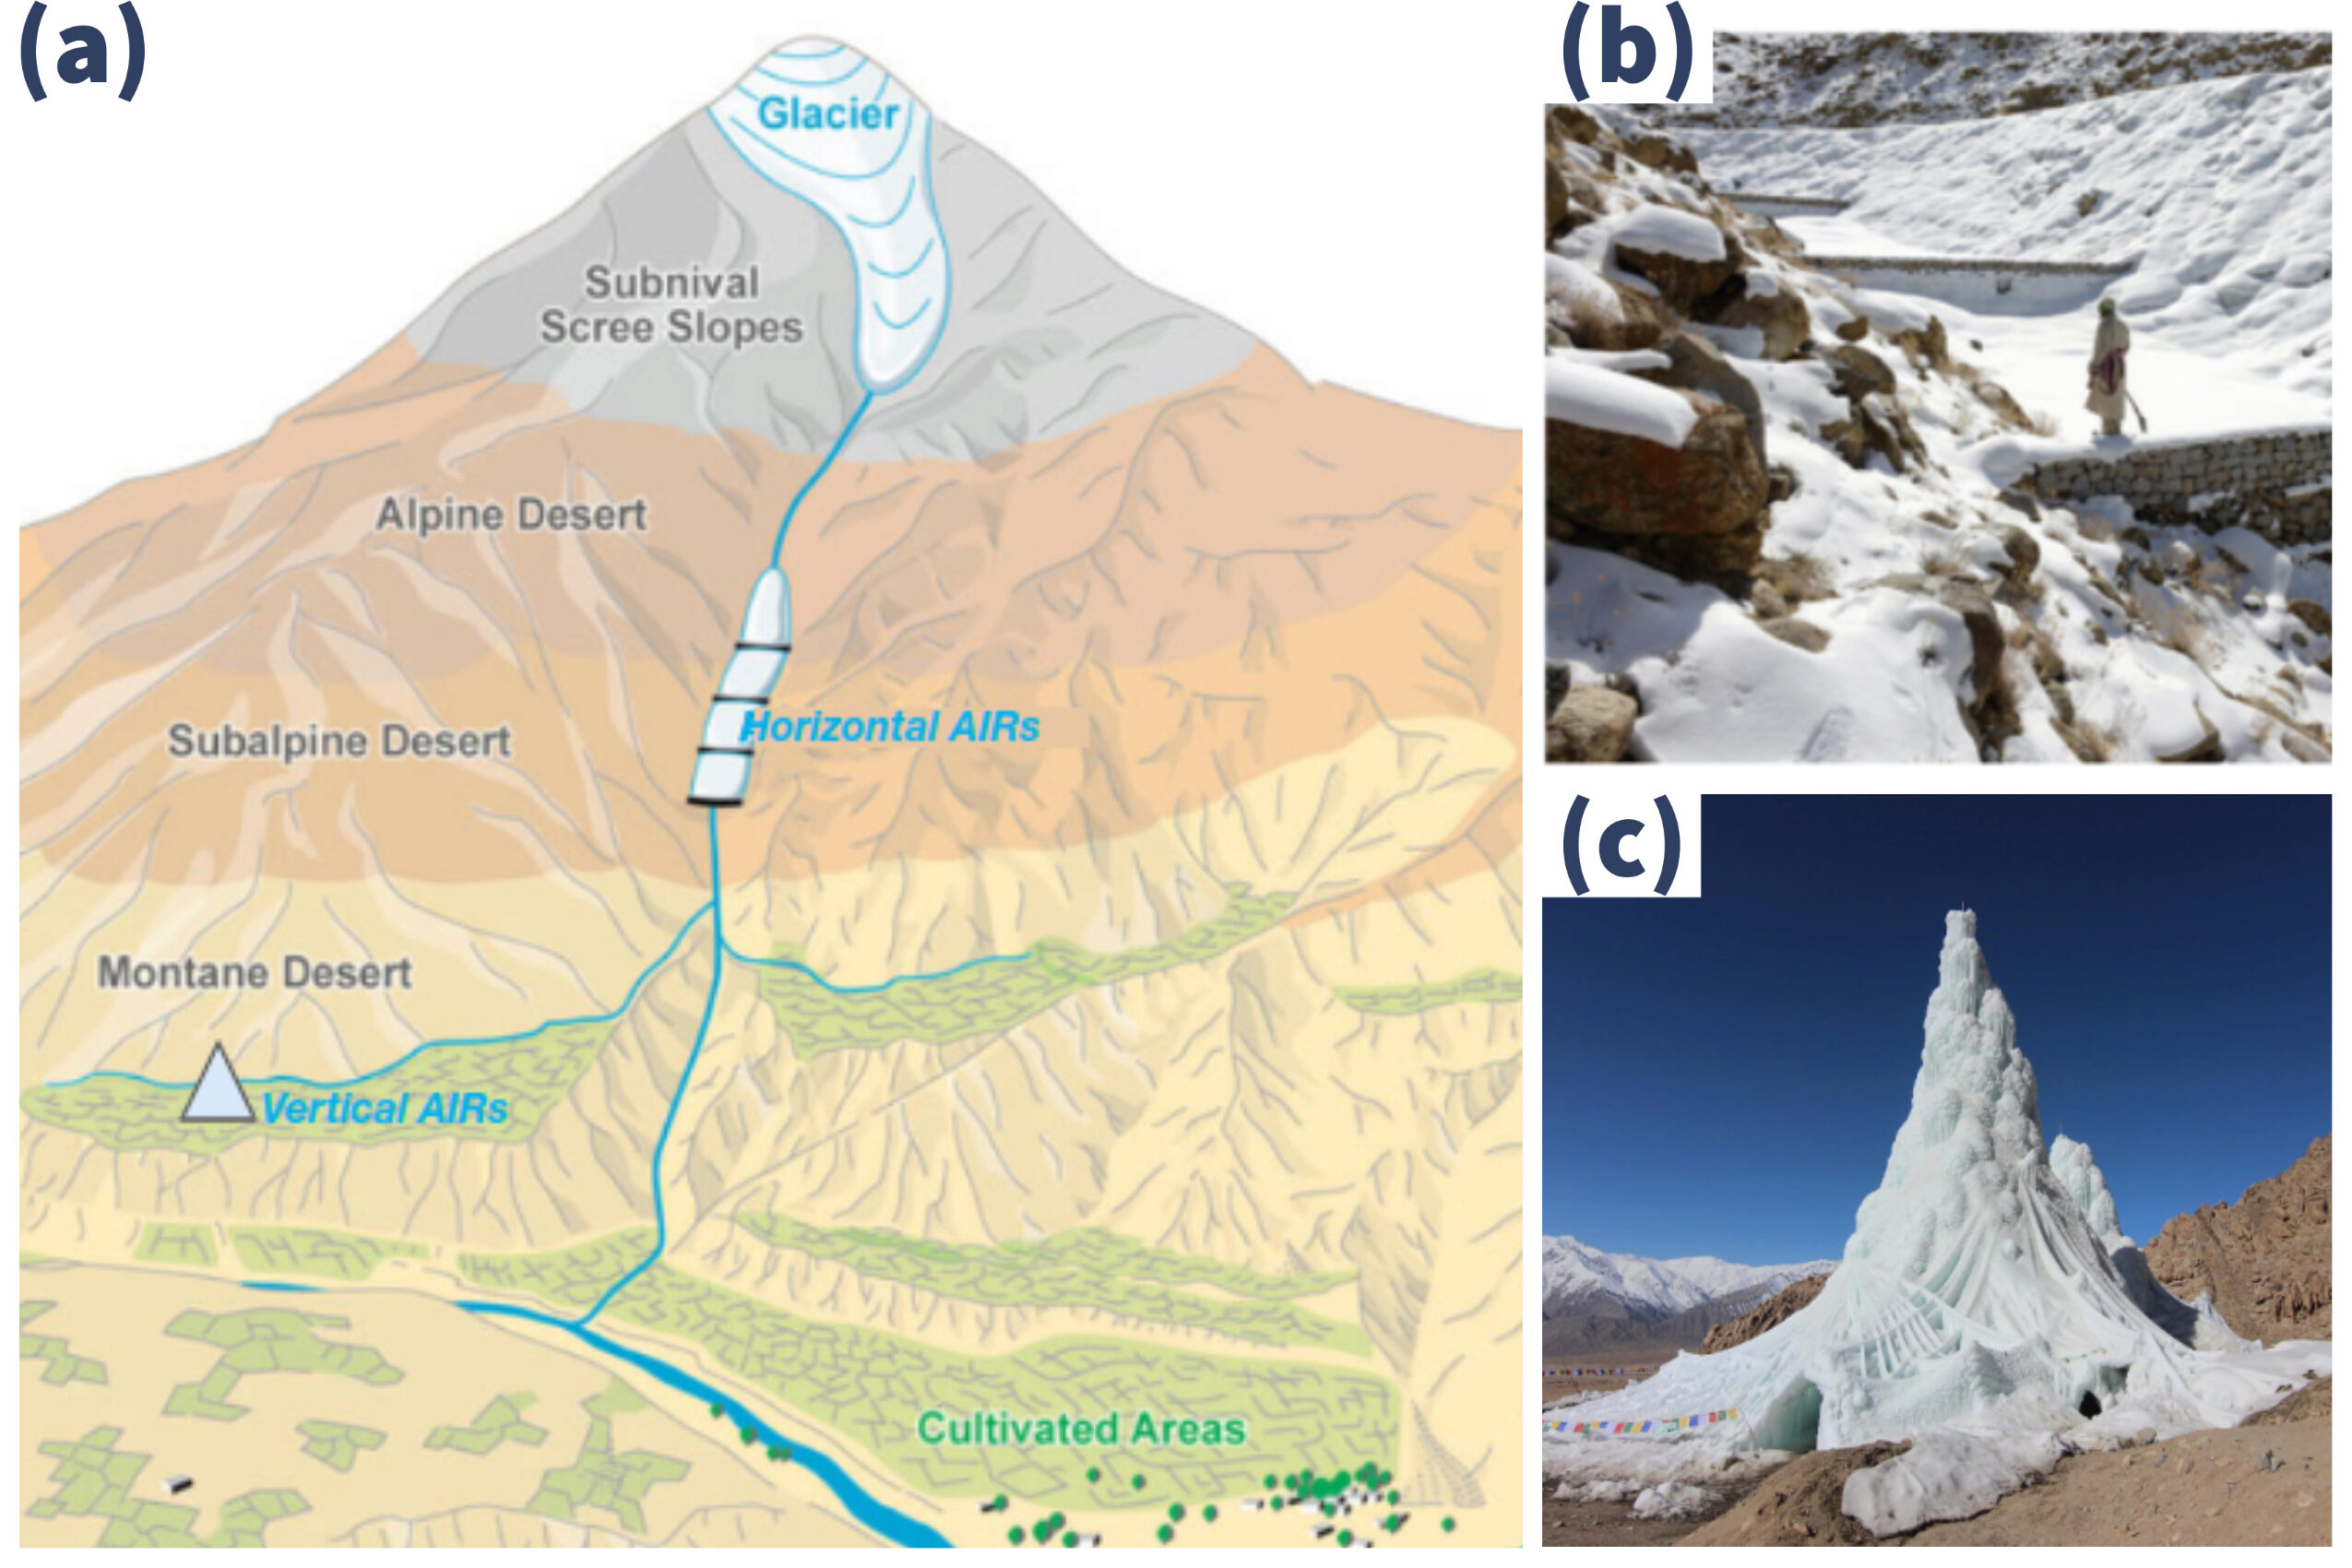
\includegraphics[width=12cm]{Figures/AIR_forms.jpg}

\caption{(a) Schematic overview of the position of artificial ice reservoirs. These constructions are located at
  altitudes between the glaciers and the irrigation networks in the cultivated areas. (b) Ice terraces at 3900
  m, located above the village of Nang, Ladakh. The cascade is composed of a series of loose masonry walls
  ranging in height from 2 to 3 $m$, which help freeze water for storage. (c) Ice stupas at 3600 m, located
above the village of Phyang, Ladakh. They are made using fountain systems. Adapted from:
\cite{nusserLocalKnowledgeGlobal2016}}

\label{fig:AIRforms}
\end{figure}

\section{Nomenclature and Classification}

In spite of the popularity of the term "artificial glacier", we deliberately use the term "ice reservoir" since
it conveys character and function of these structures more accurately
\citep{nusserSociohydrologyArtificialGlaciers2019}. Man-made ice structures typically have a lifetime in the
order of months and a size million times smaller than typical glaciers. Therefore, any comparison between these
ice structures can be misleading. Since glaciers are considered as natural ice reservoirs, we use the
terminology artificial ice reservoirs (AIRs) to distinguish man-made ice structures described in this thesis. 

A spirit of improvisation guides the construction strategy of AIRs making it difficult to classify them.
However, it has been found that construction strategies using fountain systems form AIRs which tend towards a
conical shape and those without form flat sheets of ice. Therefore, this thesis classifies all the AIRs produced
based on whether or not they use fountain systems. AIRs using fountain systems are called "ice stupas" and those
without are called "ice terraces" since this terminology denotes the resulting shape of the respective AIRs
appropriately.

\section{Objectives}

The main objective of this thesis is to quantify the water storage potential of AIRs based on the construction
site and fountain chosen. 

An integrated study approach including field measurements and modelling is applied to answer the following
research questions: 

\begin{enumerate}

\item What is the influence of construction location and fountain characteristics on AIR volume evolution? 

\item How can ice stupa fountain systems be engineered to reduce water loss and maintenance of AIRs?

\end{enumerate}

An energy and mass balance model for artificial ice reservoirs was set up to answer the first research question
(paper I and II). Since in-situ measurements were required to run this model, a measurement campaign was
executed in Switzerland and India during the past 4 winters. These datasets provided the necessary input,
calibration and validation data to model the evolution of AIRs and study their sensitivity to meteorological
conditions and fountain characterestics (paper II). 

Two weather-sensitive construction strategies were developed to answer the second research question. These
construction strategies employed fountains whose discharge rate was regulated by automation system using the AIR
model developed before. Their advantages over traditional construction strategy are quantified in paper III.

\section{Structure}

Chapter 1 introduces the motivation of this work and provides a summary of the state of knowledge about AIRs
prior to this thesis. Chapter 2 describes the origins of this technology as a religious practice. Chapter 3
gives an overview about the study sites and introduces the different field techniques applied. The influence of
the construction location through its meteorological and topographical conditions are presented in Chapter 4.
The engineering design of AIR technologies are showcased in Chapter 5 along with suggestions for their
improvement. Chapter 6 concludes the thesis with a synthesis and future outlook. Papers I, II and III are
included in the Appendix.


